\section{\LARGE{Trasformazione delle cellule di escherichia coli xl1 blue}}

\vspace{0.6cm}

\subsection{Sommario}

\subsubsection{Scopo}

L'obiettivo di questa esperienza è quello di manipolare le \textbf{culture batteriche di E.coli}
(batterio gram negativo non patogeno usato comunemente nei laboratori di ricerca),
andando a \textbf{trasportare il plasmide pUC18}, precedentemente trattato,
all'interno di questi batteri diventando cos\`i un ceppo di propagazione
(atto al clonaggio e alla propagazione di plasmidi) all'interno di un terreno di crescita.

\subsubsection{Cenni teorici}

Il procedimento di trasporto del dsDNA da esterno alla cellula all'interno è chiamato
\textbf{trasformazione batterica}, ed è un fenomeno parasessuale che consente ai batteri
lo scambio di materiale genico.

Solo alcune specie batteriche possono acquisire DNA estraneo dall'ambiente (DNA esogeno)
che deve essere a doppia elica, con facilità.
Queste sono dette cellule \textit{"naturalmente competenti"}.
Altre specie invece diventano competenti solo in particolari condizioni fisiologiche
ed altre ancora, come per esempio E.coli, necessitano di una trasformazione artificiale in
laboratorio tramite vari metodi chimici o fisici
(da noi usato è il metodo dello \textit{shock-termico}) che le rende \textbf{competenti}.

Una volta che il plasmide si trova all'interno della cellula batterica di E.coli,
la si fa crescere all'interno di piastre precedentemente preparate con LB-agar-amp
(Luria Bertani medium with ampicillin), in grado di fornire il nutrimento necessario
alla cellula per potersi nutrire e clonare,
producendo molte copie contenenti molti plasmidi ingegnerizzati di nostro interesse.

\subsection{Materiali utilizzati}

\begin{itemize}
	\item Guanti in lattice
	\item Provette Eppendorf (2mL)
	\item Micropipette (\SI{100}{\micro\liter}-\SI{1000}{\micro\liter} e \SI{2}{\micro\liter}-\SI{200}{\micro\liter})
	\item Scatola di polistirolo contenente ghiaccio
	\item Bagno termostatico
	\item Piasra di LB-agar-amp
	\item Bacchette in vetro
\end{itemize}

\subsection{Soluzioni utilizzate}

\begin{itemize}
	\item Miniprep del pUC18
	\item Cellule competenti
	\item LB liquido
\end{itemize}

\subsection{Procedimento}

\begin{enumerate}
	\item Diluire la nostra miniprep del pUC18 (descritta nell'esperienza numero 1)
  in acqua pura in misura 1:10 quindi prelevare 1$\mu$l di miniprep del pUC18 e
  9$\mu$l di acqua pura tramite una micropipetta e inserire le due componenti
  in una nuova provetta eppendorf da 2 ml. \\
  Questa diluizione \`e necessaria per avere un totale di 10$\mu$l.


	\item Prelevare in un \textit{ambiente biologicamente sterile} (sotto cappa biologica) 100 microlitri
  di cellule competenti e metterli in una provetta eppendorf da 2 ml.
  Lavorando in un ambiente sterile si garantisce la protezione da agenti inquinanti derivanti dall’esterno.

	\item Aggiungere 1$\mu$l della miniprep, diluita con acqua al passo n° 1,
  all'interno della eppendorf contenente le cellule competenti.
  In questo modo si forma una soluzione sia di cellule batteriche che di plasmidi,
  che dovranno poi entrare all'interno delle cellule.

	\item Agitare la soluzione per far s\`i che i plasmidi si distribuiscano in
  modo uniforme.
  \item Incubare la provetta contenente la soluzione in ghiaccio per una trentina di minuti
  in modo che la temperatura si abbassi gradualmente di qualche grado e che i plasmidi
  si vadano a legare sulla membrana della cellula batterica.

	\item Attendere 30' in modo che la temperatura della soluzione contenente cellule e plasmidi si è abbassi
  e stabilizzi.
  \item Ora linea teorica i plasmidi sono ancorati alle membrane delle cellule dove dovranno poi essere
  incorporati.
  \item A questo punto effettuare lo \textbf{shock termico}, portando la provetta eppendorf
  da una temperatura di ca. 0°C(ghiaccio) ad una temperatura di 42°C  molto rapidamente e lasciarla
  nel bagno termostatico per 1 minuto (la tempistica è importante poichè se si lascia il tutto ad una
  temperatura elevata per troppo tempo le cellule batteriche potrebbero morire).
  Questa operazione \`e di cruciale importanza, infatti fa in modo che sulle membrane delle cellule batteriche
  di E.coli si \textit{aprano dei pori}, permettendo il passaggio del DNA esogeno (plasmide) all'interno
  formando così una \textbf{cellula trasformata}.
	Un altro metodo per effettuare l'apertura dei pori e la successiva immissione dei plasmidi all'interno
  delle cellule competenti è l'elettroporazione che consiste in una repentina scarica elettrica
  ad alto voltaggio. Il vantaggio di questa tecnica \`e che può essere applicata anche a cellule eucariotiche.

	\begin{figure}[H]
		\centering

	  \begin{subfigure}[b]{1\textwidth}
	    \centering
	    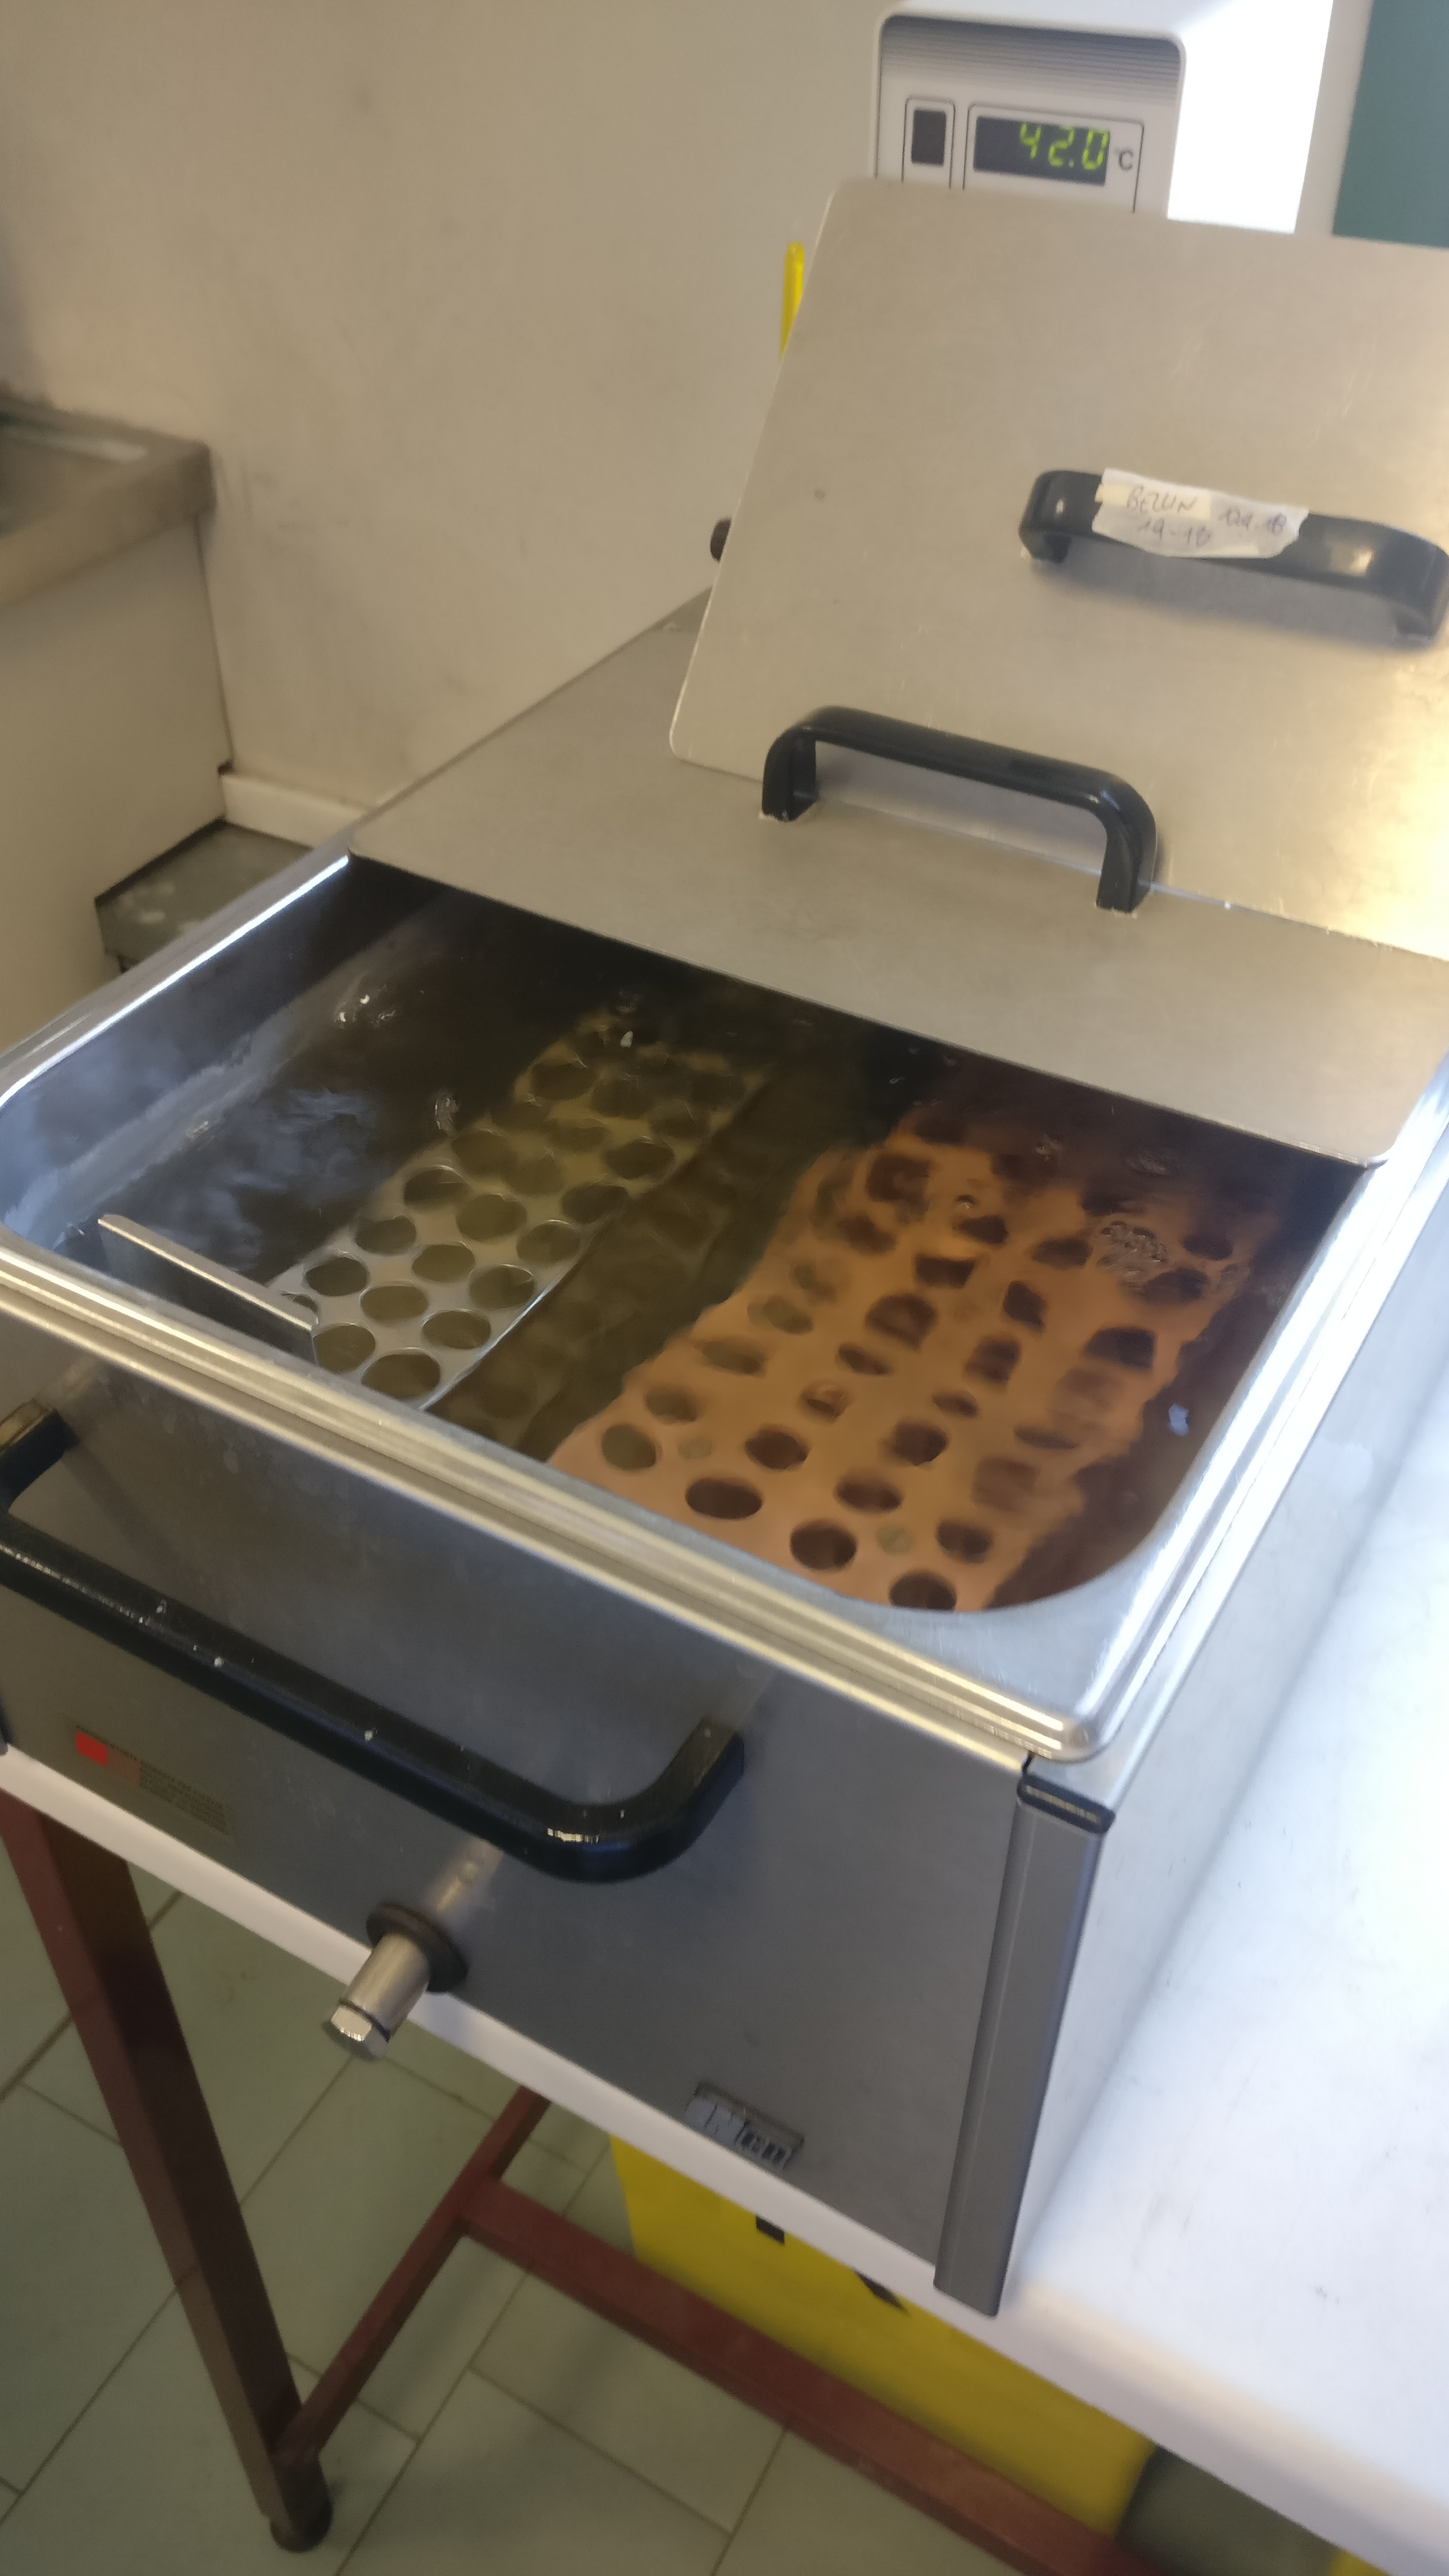
\includegraphics[width=0.3\textwidth]{./immagini/bagno_termostatico.jpg}
	    \caption{Bagno termostatico}

	  \end{subfigure}

\qquad

		\begin{subfigure}[b]{1\textwidth}
	    \centering
	    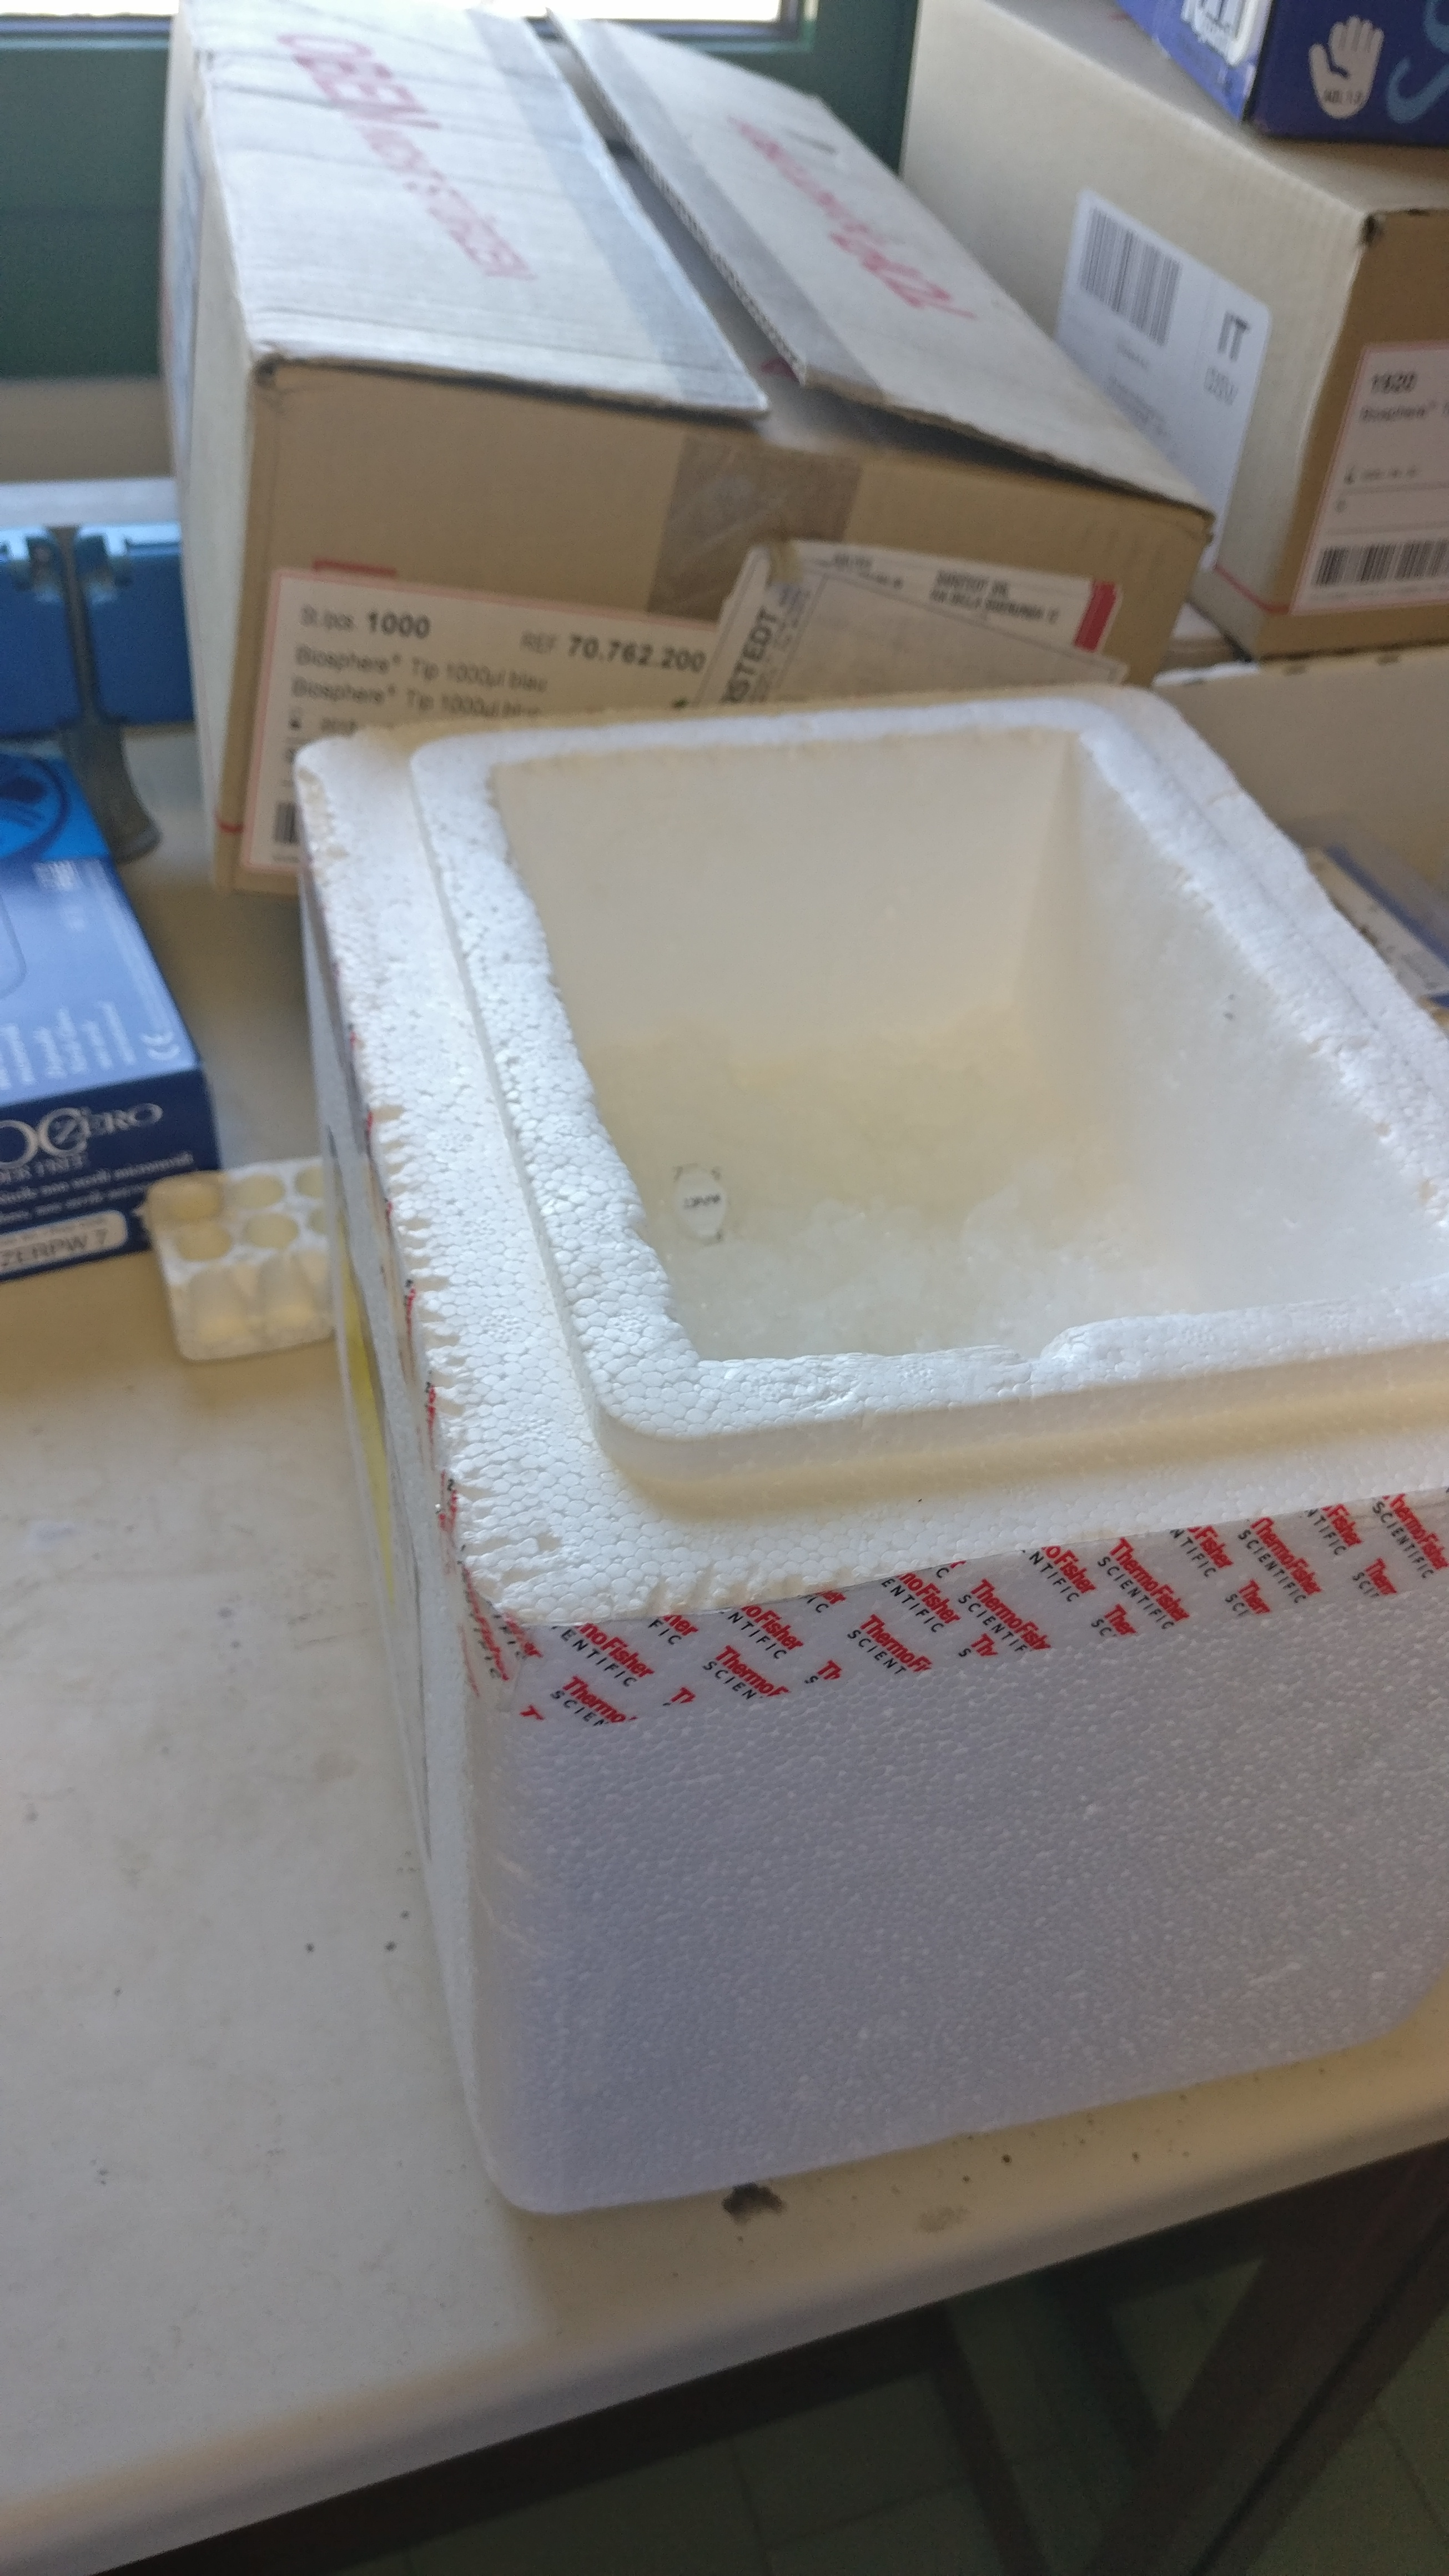
\includegraphics[width=0.3\textwidth]{./immagini/ghiaccio.jpg}
	    \caption{immersione in ghiaccio}

	  \end{subfigure}

	\end{figure}
	\item Passato un minuto prendere la eppendorf e rimetterla in ghiaccio per altri 5 minuti,
  favorendo il \textit{rallentamento del metabolismo cellulare}.
	\item Aggiungere del nutriente LB liquido all'interno della provetta, e incubarla a 37°C per 1 ora.
   In questo modo la cultura batterica si accresce e si esprime la \textbf{resistenza all'antibiotico}
   (ampicillina, codificata dal gene contenuto all'interno del plasmide).
    Una volta messo sul terreno di LB-amp, questo ci permette di sapere se il nostro plasmide è
    stato effettivamente incorporato all'interno della cellula batterica o no.
	\vspace{0.3cm}

	\begin{figure}[H]

		\centering
		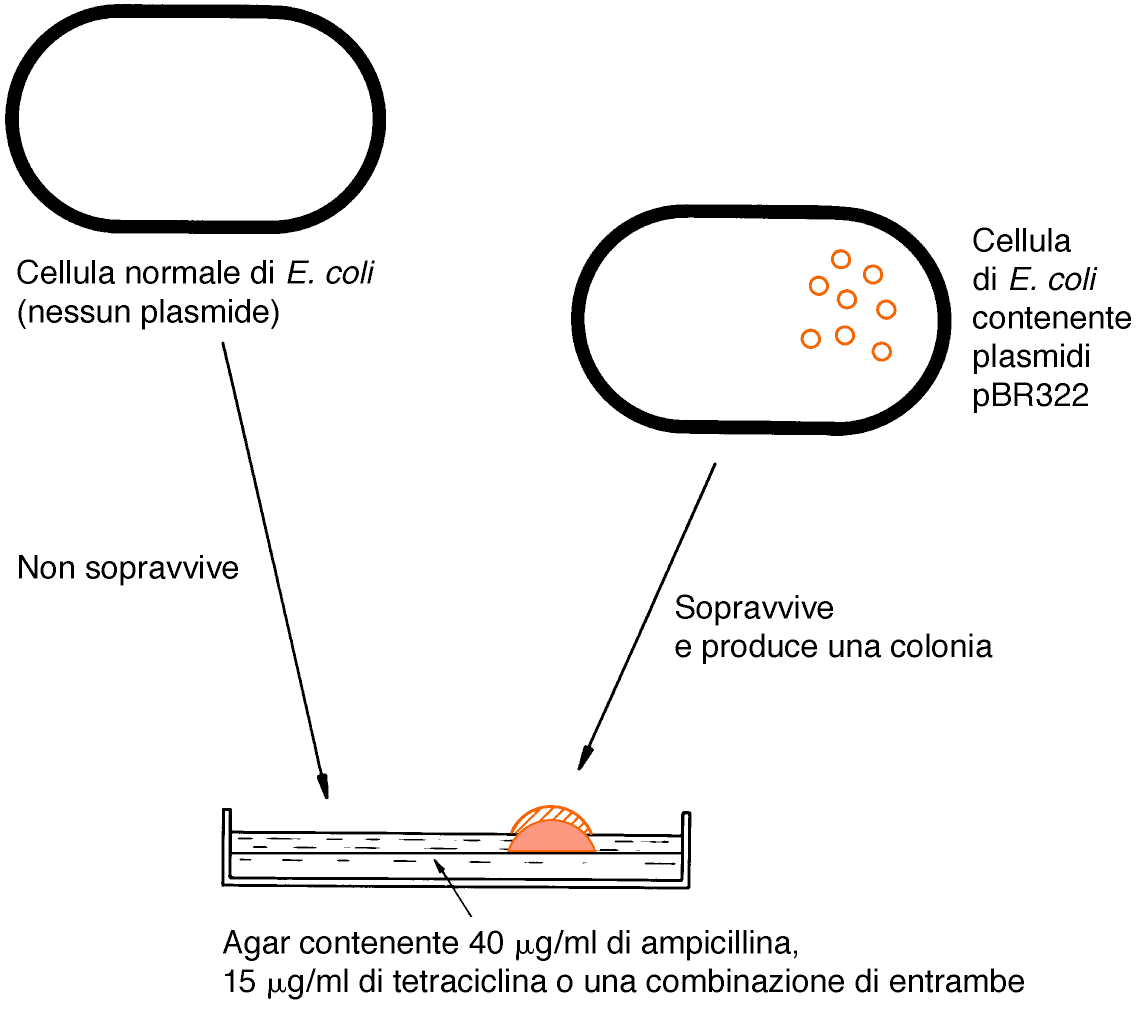
\includegraphics[width=0.6\textwidth]{./immagini/resistenza_ampicillina.png}
		\caption{Colonie con il plasmide integrato resistono al terreno con ampicillina }
		\label{resistenza ampicillina}

	\end{figure}

	\item Piastrare 150-200 microlitri della sospensione delle cellule su di una piastra di LB-amp,
  distribuendole con una bacchetta di vetro a forma di 'L' su tutta la superficie.
  Metterle poi ad una temperatura di 37°C per una notte a crescere.

	\begin{figure}[H]
		\centering
		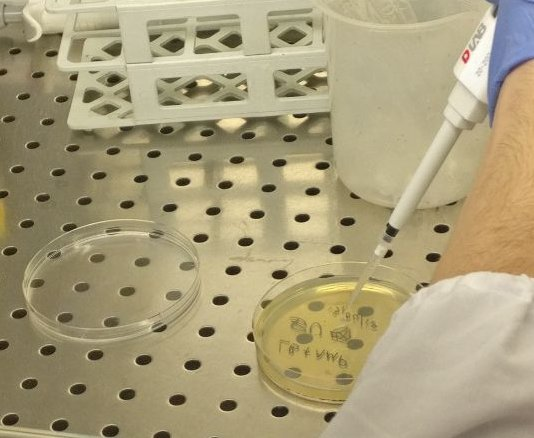
\includegraphics[width=0.6\textwidth]{./immagini/piastraggio_colonie.jpg}
		\caption{Piastraggio delle cellule di E. Coli su terreno LB-Amp}
		\label{piastraggio cellule}
	\end{figure}
\end{enumerate}

\subsection{Risultati e Conclusioni}

Tramite questa procedura abbiamo potuto inserire all'interno delle nostre cellule batteriche
di E.coli i plasmidi pUC18 rendendole competenti, permettendoci cos\`i di clonare od esprimere
i geni di interesse.
